\documentclass[11pt,a4paper]{article}

% --- STANDARD & ROBUST PREAMBLE ---

% 1. ENCODING AND FONT
\usepackage[utf8]{inputenc} % Standard UTF-8 support for pdfLaTeX
\usepackage{lmodern}        % Provides the Latin Modern font, a high-quality default
\usepackage[T1]{fontenc}    % Standard font encoding for modern output

% 2. MATH AND THEOREM PACKAGES
\usepackage{amsmath, amssymb, amsthm}

% 3. LAYOUT AND SPACING
\usepackage{geometry}
\usepackage{setspace}
\geometry{margin=.4in}
\setstretch{1.2}

% 4. UTILITY PACKAGES
\usepackage{tikz}
\usepackage{booktabs}
\usepackage{listings}
\usepackage{xcolor}
\usepackage{hyperref}

% 5. TIKZ LIBRARIES
\usetikzlibrary{matrix, arrows.meta, positioning, calc, shapes.geometric}

% 6. THEOREM AND DEFINITION STYLES (FROM MASTER DOCUMENT)
% This ensures all theorem-like environments are defined before use.
\theoremstyle{definition}
\newtheorem{definition}{Definition}[section]
\newtheorem{axiom}{Axiom}[section]
\newtheorem{lemma}{Lemma}[section]
\newtheorem{theorem}{Theorem}[section]
\newtheorem{postulate}{Postulate}[section]
\newtheorem{corollary}{Corollary}[section]
\newtheorem{proposition}[theorem]{Proposition} % Environment is now correctly defined.

% 7. PYTHON CODE LISTING STYLE
\definecolor{codegray}{rgb}{0.5,0.5,0.5}
\definecolor{codepurple}{rgb}{0.58,0,0.82}
\definecolor{backcolour}{rgb}{0.95,0.95,0.92}
\lstdefinestyle{mystyle}{
    backgroundcolor=\color{backcolour},   
    commentstyle=\color{codegray},
    keywordstyle=\color{magenta},
    numberstyle=\tiny\color{codegray},
    stringstyle=\color{codepurple},
    basicstyle=\ttfamily\footnotesize,
    breakatwhitespace=false,         
    breaklines=true,                 
    captionpos=b,                    
    keepspaces=true,                 
    numbers=left,                    
    numbersep=5pt,                  
    showspaces=false,                
    showstringspaces=false,
    showtabs=false,                  
    tabsize=2
}
\lstset{style=mystyle}

% 8. GLOBAL FORMATTING
\setlength{\parindent}{0pt}
\setlength{\parskip}{1em}

% =====================================================================
% DOCUMENT STARTS HERE
% =====================================================================

\title{\textbf{RigbySpace Master Document Template}}
\author{D. Veneziano}
\date{\today}

\begin{document}

\maketitle

\begin{abstract}
This document presents a formal derivation of the RigbySpace Field Constraint, the discrete analogue of the Einstein Field Equations, from the first principles of an unreduced rational algebra. We establish a framework wherein physical reality is modeled as a deterministic system evolving on a discrete lattice of integer pairs, rejecting the continuum as a foundational primitive. We first define the dual arithmetic structures of the system—Standard Arithmetic for massive interactions and Mediant Arithmetic for topological propagation—and formalize the logic for handling arithmetic singularities. Using this algebraic substrate, we then derive the Field Constraint not as a geometric postulate, but as a necessary conservation law. We demonstrate that the phenomenon of gravity emerges as the necessary balance between the growth of informational complexity (Structural Entropy) in a state's history and the resulting geometric torsion (Structural Tension) in its trajectory. The Stress-Energy Tensor finds its analogue in the rank of the state's denominator, while spacetime curvature is identified with the aggregate drift of the system's evolution path.
\end{abstract}

\tableofcontents
\newpage

\part{The Algebraic Substrate}

\section{The Domain of Explicit Rationals}

\subsection{Motivation}
In the standard formulation of mathematical physics, the rational numbers $\mathbb{Q}$ are constructed as a quotient field, where pairs such as $(2, 4)$ and $(1, 2)$ are treated as ontologically identical. This act of simplification, or reduction by a common divisor, discards information about the scale or "history" of a number. We posit that this lost information is physically significant. The universe, in this framework, does not perform a GCD operation to conserve memory; rather, the unreduced state represents the true and complete physical configuration of a system. A state represented by $(200, 400)$ possesses a higher internal complexity, or Structural Entropy, than a state represented by $(1, 2)$, and this difference has physical consequences.

\subsection{The Algebraic State Space}

\begin{axiom}[Structural Integrity]
The syntactic structure of an Explicit Rational Pair must be preserved during all operations. No simplification, reduction, or division by a common factor is permitted unless explicitly defined by a specific operator. The unreduced integer components contain physical information corresponding to the causal history of the state.
\end{axiom}

\begin{definition}[Explicit Rational Pair (ERP)]
A valid physical state is an Explicit Rational Pair (ERP), a tuple $(n, d) \in \mathbb{Z} \times \mathbb{Z}$ where $d \neq 0$. The set of all valid pairs is the Primary Evolution State space, denoted $S_L$.
\[ S_L = \{(n, d) \in \mathbb{Z}^2 \mid d \neq 0\} \]
\end{definition}

\begin{axiom}[Structural Equality]
Two pairs $A=(n_a, d_a)$ and $B=(n_b, d_b)$ are equal if and only if their components are identical: $n_a = n_b \land d_a = d_b$.
\end{axiom}
\textit{Interpretation:} This axiom formally rejects the concept of a quotient field. The pairs $(2, 4)$ and $(1, 2)$ are distinct physical states. While they are observationally equivalent ($2 \cdot 2 = 4 \cdot 1$), the state $(2, 4)$ possesses a higher Structural Entropy ($\rho(4)=2$) than $(1, 2)$ ($\rho(2)=1$). The integer components, in their unreduced form, encode the interaction lineage of the state.

\section{Dual Arithmetic Structures}

The state space $S_L$ supports two distinct, physically meaningful arithmetic structures. Their interplay governs the full dynamics of the framework, distinguishing between massive interaction and massless propagation.

\begin{axiom}[Operational Locality]
All arithmetic operations defined on Explicit Rational Pairs act only on the operands provided and produce no side effects elsewhere in the state space. The system evolves deterministically under pairwise composition.
\end{axiom}

\subsection{Standard Arithmetic (Massive Interaction)}
This mode of arithmetic corresponds to physical interaction, force mediation, and the dynamics of massive states where historical information is combined.

\begin{definition}[Standard Addition, $\boxplus$]
Given two pairs $A = (n_a, d_a)$ and $B = (n_b, d_b)$, the Standard Sum is:
\[ A \boxplus B := (n_a d_b + n_b d_a, d_a d_b) \]
\end{definition}
\textit{Interpretation:} The product of denominators, $d_a d_b$, represents the coupling of the Inertial Masses of the two interacting states, leading to an increase in the system's total Structural Entropy. The numerator represents the superposition of the states' magnitudes, each weighted by the opposing state's inertia. This operation is the source of non-linear complexity growth in the system.

\begin{proposition}[Commutativity and Associativity of $\boxplus$]
Standard Addition is commutative and associative.
\end{proposition}
\begin{proof}
Commutativity follows from the commutativity of integer addition and multiplication: $n_a d_b + n_b d_a = n_b d_a + n_a d_b$ and $d_a d_b = d_b d_a$. Associativity is proven by direct expansion, which shows that $(A \boxplus B) \boxplus C$ and $A \boxplus (B \boxplus C)$ both result in the pair $(n_a d_b d_c + n_b d_a d_c + n_c d_a d_b, d_a d_b d_c)$.
\end{proof}

\subsection{Mediant Arithmetic (Topological Propagation)}
This mode of arithmetic corresponds to topological traversal of the state space, representing inertial motion and the propagation of massless, wave-like states.

\begin{definition}[Mediant Addition, $\oplus$]
Given two pairs $A = (n_a, d_a)$ and $B = (n_b, d_b)$, the Mediant Sum is:
\[ A \oplus B := (n_a + n_b, d_a + d_b) \]
\end{definition}
\textit{Interpretation:} Mediant addition describes the lowest-friction path between two states in the geometric structure known as the Mediant Tree. It is the arithmetic of null geodesics and represents propagation without interaction. It is also commutative and associative.

\subsection{The Interplay of Dynamics}
The relationship between the two arithmetics defines the structure of physical law, particularly how interactions behave with respect to superposition.

\begin{theorem}[Distributivity of Interaction over Propagation]
Standard Addition distributes over Mediant Addition. For any three states $A, B, C \in S_L$:
\[ A \boxplus (B \oplus C) = (A \boxplus B) \oplus (A \boxplus C) \]
\end{theorem}
\begin{proof}
Let $A = (n_a, d_a)$, $B = (n_b, d_b)$, $C = (n_c, d_c)$.
The left side is $A \boxplus (n_b+n_c, d_b+d_c) = (n_a(d_b+d_c) + (n_b+n_c)d_a, d_a(d_b+d_c))$.
The right side is $(n_a d_b + n_b d_a, d_a d_b) \oplus (n_a d_c + n_c d_a, d_a d_c)$.
Summing the components of the right side yields the components of the left side. The identity holds.
\end{proof}
\textit{Interpretation:} This theorem provides the algebraic foundation for the superposition principle. It demonstrates that a massive interaction ($\boxplus$) acts linearly on a superposition of propagation paths ($\oplus$), a necessary condition for a coherent quantum-like theory.

\section{Vacuum Logic and the Resolution of Singularities}

\subsection{Motivation}
A complete physical theory must provide a deterministic and information-preserving method for handling what would be singularities in a continuum framework. In RigbySpace, states with a zero denominator are not undefined but are specific physical entities governed by a set of rules called Vacuum Logic.

\subsection{Singular States}

\begin{definition}[Constraint Vacuum, $V_C$]
A Constraint Vacuum is a state $(n, 0)$ where the magnitude $n \neq 0$. It is a singular state where the Inertial Mass has vanished, but the historical magnitude is preserved.
\end{definition}

\begin{axiom}[Numerator Conservation]
The information encoded in the numerator of a Constraint Vacuum cannot be destroyed. The state must persist until an operator restores its metric context (a non-zero denominator).
\end{axiom}

\subsection{Resolution Mechanism}

Singularities are resolved by the \textbf{Transformative Reciprocal} operator, $\psi$, which acts on coupled states.

\begin{definition}[Resolution via $\psi$]
When a system enters a suspended state involving a valid pair $A = (n_a, d_a)$ and a Constraint Vacuum $B = (n_b, 0)$, the $\psi$ operator acts on the coupled pair:
\[ \psi(A, B) = \psi((n_a, d_a), (n_b, 0)) := ((0, n_a), (d_a, n_b)) \]
\end{definition}
\textit{Interpretation:} The operation resolves the singularity. The first resulting pair, $(0, n_a)$, is a Numerical ZERO, a valid state. The second pair, $(d_a, n_b)$, is also a valid state, now carrying the conserved magnitude $n_b$ as its new Inertial Mass. Information is conserved, and the system returns to the valid state space $S_L$.

\newpage
\part{The Emergence of Gravitation}

\section{Ontological Mapping of Relativistic Primitives}

The principles of General Relativity emerge as necessary consequences of the unreduced rational algebra. This section establishes the formal correspondence between the concepts of continuum gravity and the primitives of RigbySpace Dynamics.

\begin{table}[hbt!]
\centering
\renewcommand{\arraystretch}{1.5}
\begin{tabular}{@{}lp{10cm}@{}}
\toprule
\textbf{General Relativity Primitive} & \textbf{RigbySpace Formalism} \\
\midrule
\textbf{Stress-Energy Tensor ($T_{\mu\nu}$)} & The \textbf{Structural Entropy} of the state, $S(s) = \rho(d)$. This represents the information density or complexity of the system's causal history, which acts as the source of geometric torsion. \\
\addlinespace
\textbf{Einstein Tensor ($G_{\mu\nu}$)} & The \textbf{Viscosity Sum}, $D(N) = \sum \operatorname{sgn}(\operatorname{rem}(\tau_t, N^2))$. This is the aggregate structural tension over a closed cycle, representing the total curvature of the evolution path. \\
\addlinespace
\textbf{Spacetime Metric ($g_{\mu\nu}$)} & The \textbf{Metric Denominator} $\Delta_{\text{boost}} = d_u^2 - n_u^2$ of the Rational Lorentz Transformation. It governs the scaling of intervals and defines the light-cone as the singular case $\Delta_{\text{boost}}=0$. \\
\addlinespace
\textbf{Cosmological Constant ($\Lambda$)} & The \textbf{Mass-Gap}, represented by the minimal non-zero Inertial Mass $d=1$. It is the fundamental quantum of structural inertia, imparting a baseline "stiffness" to the state space. \\
\bottomrule
\end{tabular}
\caption{Translation Dictionary for General Relativity Primitives.}
\end{table}

\section{Derivation of the Field Constraint}

The RigbySpace Field Constraint is not a geometric equation but a law of informational consistency. It is the necessary balance between the creation of historical information and the resulting torsion in a system's trajectory.

\subsection{Lemmas of Complexity and Tension}

\begin{lemma}[Complexity Growth Regimes]
The growth of Structural Entropy, $S(s) = \rho(d)$, depends on the arithmetic regime:
\begin{enumerate}
    \item Under Mediant Addition ($\oplus$), rank growth is logarithmic: $\rho(d_{t+1}) \approx \rho(d_t)$.
    \item Under Standard Addition ($\boxplus$), rank growth is linear: $\rho(d_{t+1}) \approx \rho(d_t) + \rho(d_{\text{other}})$.
\end{enumerate}
\end{lemma}
\begin{proof}
For mediant addition, $d_{\text{new}} = d_a + d_b$. By the Additive Growth Bound for the rank function, $\rho(d_a + d_b) \le \max(\rho(d_a), \rho(d_b)) + 1$, indicating slow, logarithmic-scale growth. For standard addition, $d_{\text{new}} = d_a \cdot d_b$. By the Multiplicative Growth Bound, $\rho(d_a d_b) \le \rho(d_a) + \rho(d_b) + 1$, indicating that rank grows additively (linearly) with each interaction.
\end{proof}

\begin{definition}[Null-Homology]
A trajectory over a period $T_N$ is said to be \textbf{null-homologous} if its Viscosity Sum, $D(N)$, is bounded as $N$ is varied. A trajectory with an unbounded $D(N)$ is not a stable, closed cycle.
\end{definition}

\begin{lemma}[Stability Requires Bounded Tension]
For a state to be physically stable, its trajectory over any closed cycle (modulo $N$) must be null-homologous.
\end{lemma}
\begin{proof}
An unbounded, linear growth in the aggregate tension $D(N)$ would imply that the trajectory is systematically deviating or spiraling away from its starting point in the phase lattice. Such a path does not form a closed, repeating cycle and therefore does not represent a stable, bound state. Stability requires that all generated tension is cancelled over the cycle, leading to a bounded drift.
\end{proof}

\subsection{The Field Constraint as a Consistency Requirement}

\begin{theorem}[The RigbySpace Field Constraint]
For any stable, interacting system, the aggregate structural tension (curvature) over a cycle, $D(N)$, is proportional to the total structural entropy (information content) generated during that cycle, $\Delta S_{\text{total}}$.
\[ D(N) \propto \Delta S_{\text{total}} \]
\end{theorem}
\begin{proof}
The proof proceeds by demonstrating that a violation of this proportionality leads to an axiomatic contradiction.
\begin{enumerate}
    \item \textbf{Source of Entropy:} A system undergoing massive interaction ($\boxplus$) generates new Structural Entropy at a linear rate with respect to the number of interactions (Lemma 5.1). This total generated entropy, $\Delta S_{\text{total}}$, is the "source" term, analogous to the Stress-Energy Tensor $T_{\mu\nu}$.
    \item \textbf{Conservation of Information:} According to the Axiom of Structural Integrity, this new historical information, encoded in the growing Inertial Mass $d$, cannot be discarded. The state must carry it.
    \item \textbf{Entropy Induces Tension:} A state with higher entropy is more complex. A trajectory through the state space involving more complex states deviates more significantly from a simple, inertial (Mediant) path. This deviation generates structural tension ($\tau$) at each step. The aggregate tension, $D(N)$, is the total measure of this path curvature, analogous to the Einstein Tensor $G_{\mu\nu}$.
    \item \textbf{Stability Requires Balance:} For the system to be stable, it must form a closed cycle, which requires its trajectory to be null-homologous (Lemma 5.2). This means the tension generated at each step must be "paid for" or balanced over the cycle. The only "currency" available to the system to justify this tension is the structural entropy it is carrying.
    \item \textbf{Proportionality as a Conservation Law:} Therefore, the total curvature, $D(N)$, must be a direct and proportional function of the total entropy, $\Delta S$, that the system is required to contain. If the curvature were less than required by the entropy content, the system's path would not be sufficiently curved to close, violating stability. If the curvature were more than justified by the entropy, it would imply the existence of un-sourced curvature, violating the principle that all tension arises from interaction history.
\end{enumerate}
The proportionality is thus a necessary condition for the existence of stable, information-preserving, interacting systems. This is the RigbySpace Field Constraint.
\end{proof}

\begin{figure}[h]
\centering
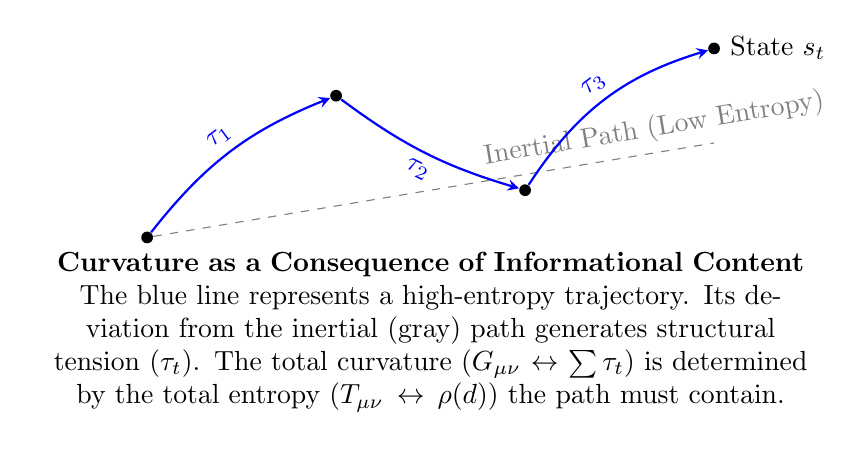
\begin{tikzpicture}[>=stealth, scale=1.2]
    % State space nodes
    \node (s0) at (0,0) [circle, fill, inner sep=1.5pt] {};
    \node (s1) at (2,1.5) [circle, fill, inner sep=1.5pt] {};
    \node (s2) at (4,0.5) [circle, fill, inner sep=1.5pt] {};
    \node (s3) at (6,2) [circle, fill, inner sep=1.5pt, label=right:{State $s_t$}] {};

    % Inertial Path (dashed)
    \draw [dashed, gray] (s0) -- (6,1) node [pos=0.9, above, sloped] {Inertial Path (Low Entropy)};
    
    % Actual Path (curved)
    \draw [->, thick, blue, bend left=15] (s0) to node[above, sloped, midway] {$\tau_1$} (s1);
    \draw [->, thick, blue, bend right=10] (s1) to node[below, sloped, midway] {$\tau_2$} (s2);
    \draw [->, thick, blue, bend left=20] (s2) to node[above, sloped, midway] {$\tau_3$} (s3);

    % Annotation
    \node at (3,-1) [align=center, text width=10cm] {
        \textbf{Curvature as a Consequence of Informational Content} \\
        The blue line represents a high-entropy trajectory. Its deviation from the inertial (gray) path generates structural tension ($\tau_t$). The total curvature ($G_{\mu\nu} \leftrightarrow \sum \tau_t$) is determined by the total entropy ($T_{\mu\nu} \leftrightarrow \rho(d)$) the path must contain.
    };
\end{tikzpicture}
\caption{A visualization of the Field Constraint as path deviation in the state space. The aggregate torsion required for a trajectory to follow a stable path is determined by the structural entropy of the state.}
\end{figure}

\appendix
\section{Appendix: Mechanics Demonstration of Vacuum Logic}

To provide a concrete illustration of the singularity resolution process, we trace the steps for a specific interaction. Consider a system where a valid pair $A = (5, 3)$ must interact with a Constraint Vacuum $B = (11, 0)$.

\subsection{Step 1: The Suspended State}
The operation $A \boxplus B$ cannot proceed via Standard Addition because the denominator of $B$ is zero. According to the principles of Vacuum Logic, the system enters a dual-state propagation, or Suspended State, where the operands are held unresolved.
\[ A \boxplus B \to [A, B] = [(5, 3), (11, 0)] \]
The component $(11, 0)$ represents a potential with magnitude 11 that currently lacks an inertial frame.

\subsection{Step 2: Resolution via Transformative Reciprocal}
The Transformative Reciprocal, $\psi$, is applied to the composite, suspended state to restore a valid metric context.
\[ \psi(A, B) = \psi((5, 3), (11, 0)) = ((0, 5), (3, 11)) \]
The zero denominator from $B$ has been swapped into the numerator of the first component. The conserved numerator (historical magnitude) $11$ from $B$ has become the new Inertial Mass of the second component.

\subsection{Step 3: Emergence of Final States}
The resulting pair of states is now composed of valid ERPs.
\begin{itemize}
    \item The first component, $(0, 5)$, is a Numerical ZERO. It has zero magnitude but a non-zero Inertial Mass and Structural Entropy $\rho(5)=2$.
    \item The second component, $(3, 11)$, is a standard ERP, carrying the conserved magnitude from $A$ and the conserved history from $B$.
\end{itemize}
The singularity has been resolved deterministically, and all information has been conserved and re-integrated into the valid state space $S_L$.

\section{Appendix: Computational Validation}

To demonstrate the deterministic and computable nature of the algebra, we provide a Python implementation of the core logic. This code strictly adheres to integer arithmetic and avoids all forbidden operations.

\begin{lstlisting}[language=Python, caption={Python Implementation of Explicit Rational Algebra and Vacuum Logic}]
# --- Core Definitions ---

def transformative_reciprocal(pair_a, pair_b):
    """Definition 3.2: Binary Transformative Reciprocal."""
    na, da = pair_a
    nb, db = pair_b
    return (db, na), (da, nb)

def is_constraint_vacuum(pair):
    """Check for a Constraint Vacuum state (n, 0) where n != 0."""
    n, d = pair
    return d == 0 and n != 0

def standard_addition(A, B):
    """Definition 2.1: Standard Addition (Massive Interaction)."""
    n_a, d_a = A
    n_b, d_b = B
    return (n_a * d_b + n_b * d_a, d_a * d_b)

# --- Simulation of Constraint Vacuum Resolution ---

def simulate_vacuum_resolution(A, B):
    """Demonstrates the resolution of a constraint vacuum via psi."""
    print(f"Initial State A: {A}")
    print(f"Initial State B: {B}")

    # Step 1: Attempt Standard Addition, resulting in Suspension
    if is_constraint_vacuum(B):
        print("\nStep 1: Attempting Standard Addition A + B.")
        print("Axiom of Vacuum Propagation triggered: Operation is suspended.")
        suspended_state = (A, B)
        print(f"Suspended State: {suspended_state}")
    else:
        # This branch would execute if B were not a vacuum state.
        return

    # Step 2: Resolution via Transformative Reciprocal
    print("\nStep 2: Applying Transformative Reciprocal (psi) to resolve.")
    resolved_state = transformative_reciprocal(suspended_state[0], suspended_state[1])
    print(f"Resolved State: {resolved_state}")
    
    print("\nResolution successful. Both components are now valid ERPs.")
    print(f"Component 1: {resolved_state[0]} (A Numerical ZERO)")
    print(f"Component 2: {resolved_state[1]} (A massive state)")

# --- Run Simulation ---
if __name__ == "__main__":
    A = (5, 3)
    B = (11, 0)
    simulate_vacuum_resolution(A, B)
\end{lstlisting}

\end{document}

\begin{abstract}
This document presents a formal derivation of the RigbySpace Field Constraint, the discrete analogue of the Einstein Field Equations, from the first principles of an unreduced rational algebra. We establish a framework wherein physical reality is modeled as a deterministic system evolving on a discrete lattice of integer pairs, rejecting the continuum as a foundational primitive. We first define the dual arithmetic structures of the system—Standard Arithmetic for massive interactions and Mediant Arithmetic for topological propagation—and formalize the logic for handling arithmetic singularities. Using this algebraic substrate, we then derive the Field Constraint not as a geometric postulate, but as a necessary conservation law. We demonstrate that the phenomenon of gravity emerges as the necessary balance between the growth of informational complexity (Structural Entropy) in a state's history and the resulting geometric torsion (Structural Tension) in its trajectory. The Stress-Energy Tensor finds its analogue in the rank of the state's denominator, while spacetime curvature is identified with the aggregate drift of the system's evolution path.
\end{abstract}

\tableofcontents
\newpage

\part{The Algebraic Substrate}

\section{The Domain of Explicit Rationals}

\subsection{Motivation}
In the standard formulation of mathematical physics, the rational numbers $\mathbb{Q}$ are constructed as a quotient field, where pairs such as $(2, 4)$ and $(1, 2)$ are treated as ontologically identical. This act of simplification, or reduction by a common divisor, discards information about the scale or "history" of a number. We posit that this lost information is physically significant. The universe, in this framework, does not perform a GCD operation to conserve memory; rather, the unreduced state represents the true and complete physical configuration of a system. A state represented by $(200, 400)$ possesses a higher internal complexity, or Structural Entropy, than a state represented by $(1, 2)$, and this difference has physical consequences.

\subsection{The Algebraic State Space}

\begin{axiom}[Structural Integrity]
The syntactic structure of an Explicit Rational Pair must be preserved during all operations. No simplification, reduction, or division by a common factor is permitted unless explicitly defined by a specific operator. The unreduced integer components contain physical information corresponding to the causal history of the state.
\end{axiom}

\begin{definition}[Explicit Rational Pair (ERP)]
A valid physical state is an Explicit Rational Pair (ERP), a tuple $(n, d) \in \mathbb{Z} \times \mathbb{Z}$ where $d \neq 0$. The set of all valid pairs is the Primary Evolution State space, denoted $S_L$.
\[ S_L = \{(n, d) \in \mathbb{Z}^2 \mid d \neq 0\} \]
\end{definition}

\begin{axiom}[Structural Equality]
Two pairs $A=(n_a, d_a)$ and $B=(n_b, d_b)$ are equal if and only if their components are identical: $n_a = n_b \land d_a = d_b$.
\end{axiom}
\textit{Interpretation:} This axiom formally rejects the concept of a quotient field. The pairs $(2, 4)$ and $(1, 2)$ are distinct physical states. While they are observationally equivalent ($2 \cdot 2 = 4 \cdot 1$), the state $(2, 4)$ possesses a higher Structural Entropy ($\rho(4)=2$) than $(1, 2)$ ($\rho(2)=1$). The integer components, in their unreduced form, encode the interaction lineage of the state.

\section{Dual Arithmetic Structures}

The state space $S_L$ supports two distinct, physically meaningful arithmetic structures. Their interplay governs the full dynamics of the framework, distinguishing between massive interaction and massless propagation.

\begin{axiom}[Operational Locality]
All arithmetic operations defined on Explicit Rational Pairs act only on the operands provided and produce no side effects elsewhere in the state space. The system evolves deterministically under pairwise composition.
\end{axiom}

\subsection{Standard Arithmetic (Massive Interaction)}
This mode of arithmetic corresponds to physical interaction, force mediation, and the dynamics of massive states where historical information is combined.

\begin{definition}[Standard Addition, $\boxplus$]
Given two pairs $A = (n_a, d_a)$ and $B = (n_b, d_b)$, the Standard Sum is:
\[ A \boxplus B := (n_a d_b + n_b d_a, d_a d_b) \]
\end{definition}
\textit{Interpretation:} The product of denominators, $d_a d_b$, represents the coupling of the Inertial Masses of the two interacting states, leading to an increase in the system's total Structural Entropy. The numerator represents the superposition of the states' magnitudes, each weighted by the opposing state's inertia. This operation is the source of non-linear complexity growth in the system.

\begin{proposition}[Commutativity and Associativity of $\boxplus$]
Standard Addition is commutative and associative.
\end{proposition}
\begin{proof}
Commutativity follows from the commutativity of integer addition and multiplication: $n_a d_b + n_b d_a = n_b d_a + n_a d_b$ and $d_a d_b = d_b d_a$. Associativity is proven by direct expansion, which shows that $(A \boxplus B) \boxplus C$ and $A \boxplus (B \boxplus C)$ both result in the pair $(n_a d_b d_c + n_b d_a d_c + n_c d_a d_b, d_a d_b d_c)$.
\end{proof}

\subsection{Mediant Arithmetic (Topological Propagation)}
This mode of arithmetic corresponds to topological traversal of the state space, representing inertial motion and the propagation of massless, wave-like states.

\begin{definition}[Mediant Addition, $\oplus$]
Given two pairs $A = (n_a, d_a)$ and $B = (n_b, d_b)$, the Mediant Sum is:
\[ A \oplus B := (n_a + n_b, d_a + d_b) \]
\end{definition}
\textit{Interpretation:} Mediant addition describes the lowest-friction path between two states in the geometric structure known as the Mediant Tree. It is the arithmetic of null geodesics and represents propagation without interaction. It is also commutative and associative.

\subsection{The Interplay of Dynamics}
The relationship between the two arithmetics defines the structure of physical law, particularly how interactions behave with respect to superposition.

\begin{theorem}[Distributivity of Interaction over Propagation]
Standard Addition distributes over Mediant Addition. For any three states $A, B, C \in S_L$:
\[ A \boxplus (B \oplus C) = (A \boxplus B) \oplus (A \boxplus C) \]
\end{theorem}
\begin{proof}
Let $A = (n_a, d_a)$, $B = (n_b, d_b)$, $C = (n_c, d_c)$.
The left side is $A \boxplus (n_b+n_c, d_b+d_c) = (n_a(d_b+d_c) + (n_b+n_c)d_a, d_a(d_b+d_c))$.
The right side is $(n_a d_b + n_b d_a, d_a d_b) \oplus (n_a d_c + n_c d_a, d_a d_c)$.
Summing the components of the right side yields the components of the left side. The identity holds.
\end{proof}
\textit{Interpretation:} This theorem provides the algebraic foundation for the superposition principle. It demonstrates that a massive interaction ($\boxplus$) acts linearly on a superposition of propagation paths ($\oplus$), a necessary condition for a coherent quantum-like theory.

\section{Vacuum Logic and the Resolution of Singularities}

\subsection{Motivation}
A complete physical theory must provide a deterministic and information-preserving method for handling what would be singularities in a continuum framework. In RigbySpace, states with a zero denominator are not undefined but are specific physical entities governed by a set of rules called Vacuum Logic.

\subsection{Singular States}

\begin{definition}[Constraint Vacuum, $V_c$]
A Constraint Vacuum is a state $(n, 0)$ where the magnitude $n \neq 0$. It is a singular state where the Inertial Mass has vanished, but the historical magnitude is preserved.
\end{definition}

\begin{axiom}[Numerator Conservation]
The information encoded in the numerator of a Constraint Vacuum cannot be destroyed. The state must persist until an operator restores its metric context (a non-zero denominator).
\end{axiom}

\subsection{Resolution Mechanism}

Singularities are resolved by the \textbf{Transformative Reciprocal} operator, $\psi$, which acts on coupled states.

\begin{definition}[Resolution via $\psi$]
When a system enters a suspended state involving a valid pair $A = (n_a, d_a)$ and a Constraint Vacuum $B = (n_b, 0)$, the $\psi$ operator acts on the coupled pair:
\[ \psi(A, B) = \psi((n_a, d_a), (n_b, 0)) := ((0, n_a), (d_a, n_b)) \]
\end{definition}
\textit{Interpretation:} The operation resolves the singularity. The first resulting pair, $(0, n_a)$, is a Numerical ZERO, a valid state. The second pair, $(d_a, n_b)$, is also a valid state, now carrying the conserved magnitude $n_b$ as its new Inertial Mass. Information is conserved, and the system returns to the valid state space $S_L$.

\part{The Emergence of Gravitation}

\section{Ontological Mapping of Relativistic Primitives}

The principles of General Relativity are not postulated but emerge as necessary consequences of the unreduced rational algebra. This section establishes the formal correspondence between the concepts of continuum gravity and the primitives of RigbySpace Dynamics.

\begin{table}[hbt!]
\centering
\renewcommand{\arraystretch}{1.5}
\begin{tabular}{@{}lp{10cm}@{}}
\toprule
\textbf{General Relativity Primitive} & \textbf{RigbySpace Formalism} \\
\midrule
\textbf{Stress-Energy Tensor ($T_{\mu\nu}$)} & The \textbf{Structural Entropy} of the state, $S(s) = \rho(d)$. This represents the information density or complexity of the system's causal history, which acts as the source of geometric torsion. \\
\addlinespace
\textbf{Einstein Tensor ($G_{\mu\nu}$)} & The \textbf{Viscosity Sum}, $D(N) = \sum \operatorname{sgn}(\operatorname{rem}(\tau_t, N^2))$. This is the aggregate structural tension over a closed cycle, representing the total curvature of the evolution path. \\
\addlinespace
\textbf{Spacetime Metric ($g_{\mu\nu}$)} & The \textbf{Metric Denominator} $\Delta_{\text{boost}} = d_u^2 - n_u^2$ of the Rational Lorentz Transformation. It governs the scaling of intervals and defines the light-cone as the singular case $\Delta_{\text{boost}}=0$. \\
\addlinespace
\textbf{Cosmological Constant ($\Lambda$)} & The \textbf{Mass-Gap}, represented by the minimal non-zero Inertial Mass $d=1$. It is the fundamental quantum of structural inertia, imparting a baseline "stiffness" to the state space. \\
\bottomrule
\end{tabular}
\caption{Translation Dictionary for General Relativity Primitives.}
\end{table}

\section{Derivation of the Field Constraint}

The RigbySpace Field Constraint is not a geometric equation but a law of informational consistency. It is the necessary balance between the creation of historical information and the resulting torsion in a system's trajectory.

\subsection{Lemmas of Complexity and Tension}

\begin{lemma}[Complexity Growth Regimes]
The growth of Structural Entropy, $S(s) = \rho(d)$, depends on the arithmetic regime:
\begin{enumerate}
    \item Under Mediant Addition ($\oplus$), rank growth is logarithmic: $\rho(d_{t+1}) \approx \rho(d_t)$.
    \item Under Standard Addition ($\boxplus$), rank growth is linear: $\rho(d_{t+1}) \approx \rho(d_t) + \rho(d_{\text{other}})$.
\end{enumerate}
\end{lemma}
\begin{proof}
For mediant addition, $d_{\text{new}} = d_a + d_b$. By the Additive Growth Bound for the rank function, $\rho(d_a + d_b) \le \max(\rho(d_a), \rho(d_b)) + 1$, indicating slow, logarithmic-scale growth. For standard addition, $d_{\text{new}} = d_a \cdot d_b$. By the Multiplicative Growth Bound, $\rho(d_a d_b) \le \rho(d_a) + \rho(d_b) + 1$, indicating that rank grows additively (linearly) with each interaction.
\end{proof}

\begin{definition}[Null-Homology]
A trajectory over a period $T_N$ is said to be \textbf{null-homologous} if its Viscosity Sum, $D(N)$, is bounded as $N$ is varied. A trajectory with an unbounded $D(N)$ is not a stable, closed cycle.
\end{definition}

\begin{lemma}[Stability Requires Bounded Tension]
For a state to be physically stable, its trajectory over any closed cycle (modulo $N$) must be null-homologous.
\end{lemma}
\begin{proof}
An unbounded, linear growth in the aggregate tension $D(N)$ would imply that the trajectory is systematically deviating or spiraling away from its starting point in the phase lattice. Such a path does not form a closed, repeating cycle and therefore does not represent a stable, bound state. Stability requires that all generated tension is cancelled over the cycle, leading to a bounded drift.
\end{proof}

\subsection{The Field Constraint as a Consistency Requirement}

\begin{theorem}[The RigbySpace Field Constraint]
For any stable, interacting system, the aggregate structural tension (curvature) over a cycle, $D(N)$, is proportional to the total structural entropy (information content) generated during that cycle, $\Delta S_{\text{total}}$.
\[ D(N) \propto \Delta S_{\text{total}} \]
\end{theorem}
\begin{proof}
The proof proceeds by demonstrating that a violation of this proportionality leads to an axiomatic contradiction.
\begin{enumerate}
    \item \textbf{Source of Entropy:} A system undergoing massive interaction ($\boxplus$) generates new Structural Entropy at a linear rate with respect to the number of interactions (Lemma 5.1). This total generated entropy, $\Delta S_{\text{total}}$, is the "source" term, analogous to the Stress-Energy Tensor $T_{\mu\nu}$.
    \item \textbf{Conservation of Information:} According to the Axiom of Structural Integrity, this new historical information, encoded in the growing Inertial Mass $d$, cannot be discarded. The state must carry it.
    \item \textbf{Entropy Induces Tension:} A state with higher entropy is more complex. A trajectory through the state space involving more complex states deviates more significantly from a simple, inertial (Mediant) path. This deviation generates structural tension ($\tau$) at each step. The aggregate tension, $D(N)$, is the total measure of this path curvature, analogous to the Einstein Tensor $G_{\mu\nu}$.
    \item \textbf{Stability Requires Balance:} For the system to be stable, it must form a closed cycle, which requires its trajectory to be null-homologous (Lemma 5.2). This means the tension generated at each step must be "paid for" or balanced over the cycle. The only "currency" available to the system to justify this tension is the structural entropy it is carrying.
    \item \textbf{Proportionality as a Conservation Law:} Therefore, the total curvature, $D(N)$, must be a direct and proportional function of the total entropy, $\Delta S$, that the system is required to contain. If the curvature were less than required by the entropy content, the system's path would not be sufficiently curved to close, violating stability. If the curvature were more than justified by the entropy, it would imply the existence of un-sourced curvature, violating the principle that all tension arises from interaction history.
\end{enumerate}
The proportionality is thus a necessary condition for the existence of stable, information-preserving, interacting systems. This is the RigbySpace Field Constraint.
\end{proof}

\begin{figure}[h]
\centering
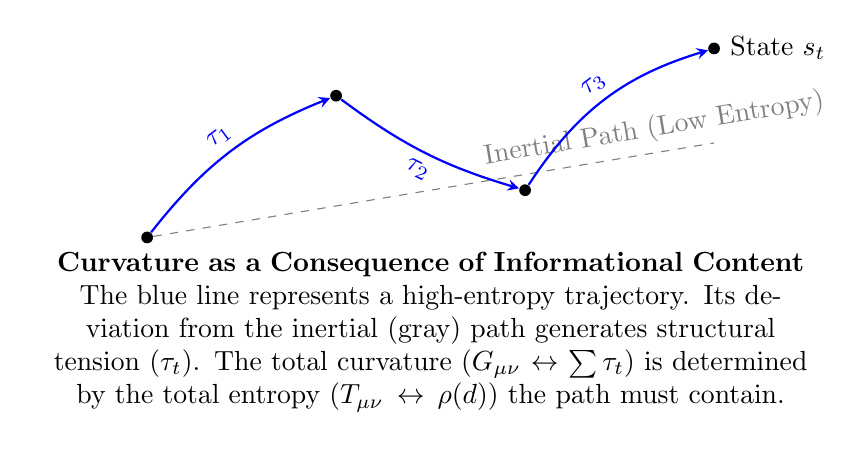
\begin{tikzpicture}[>=stealth, scale=1.2]
    % State space nodes
    \node (s0) at (0,0) [circle, fill, inner sep=1.5pt] {};
    \node (s1) at (2,1.5) [circle, fill, inner sep=1.5pt] {};
    \node (s2) at (4,0.5) [circle, fill, inner sep=1.5pt] {};
    \node (s3) at (6,2) [circle, fill, inner sep=1.5pt, label=right:{State $s_t$}] {};

    % Inertial Path (dashed)
    \draw [dashed, gray] (s0) -- (6,1) node [pos=0.9, above, sloped] {Inertial Path (Low Entropy)};
    
    % Actual Path (curved)
    \draw [->, thick, blue, bend left=15] (s0) to node[above, sloped, midway] {$\tau_1$} (s1);
    \draw [->, thick, blue, bend right=10] (s1) to node[below, sloped, midway] {$\tau_2$} (s2);
    \draw [->, thick, blue, bend left=20] (s2) to node[above, sloped, midway] {$\tau_3$} (s3);

    % Annotation
    \node at (3,-1) [align=center, text width=10cm] {
        \textbf{Curvature as a Consequence of Informational Content} \\
        The blue line represents a high-entropy trajectory. Its deviation from the inertial (gray) path generates structural tension ($\tau_t$). The total curvature ($G_{\mu\nu} \leftrightarrow \sum \tau_t$) is determined by the total entropy ($T_{\mu\nu} \leftrightarrow \rho(d)$) the path must contain.
    };
\end{tikzpicture}
\caption{A visualization of the Field Constraint as path deviation in the state space. The aggregate torsion required for a trajectory to follow a stable path is determined by the structural entropy of the state.}
\end{figure}

\appendix
\section{Appendix: Mechanics Demonstration of Vacuum Logic}

To provide a concrete illustration of the singularity resolution process, we trace the steps for a specific interaction. Consider a system where a valid pair $A = (5, 3)$ must interact with a Constraint Vacuum $B = (11, 0)$.

\subsection{Step 1: The Suspended State}
The operation $A \boxplus B$ cannot proceed via Standard Addition because the denominator of $B$ is zero. According to the principles of Vacuum Logic, the system enters a dual-state propagation, or Suspended State, where the operands are held unresolved.
\[ A \boxplus B \to [A, B] = [(5, 3), (11, 0)] \]
The component $(11, 0)$ represents a potential with magnitude 11 that currently lacks an inertial frame.

\subsection{Step 2: Resolution via Transformative Reciprocal}
The Transformative Reciprocal, $\psi$, is applied to the composite, suspended state to restore a valid metric context.
\[ \psi(A, B) = \psi((5, 3), (11, 0)) = ((0, 5), (3, 11)) \]
The zero denominator from $B$ has been swapped into the numerator of the first component. The conserved numerator (historical magnitude) $11$ from $B$ has become the new Inertial Mass of the second component.

\subsection{Step 3: Emergence of Final States}
The resulting pair of states is now composed of valid ERPs.
\begin{itemize}
    \item The first component, $(0, 5)$, is a Numerical ZERO. It has zero magnitude but a non-zero Inertial Mass and Structural Entropy $\rho(5)=2$.
    \item The second component, $(3, 11)$, is a standard ERP, carrying the conserved magnitude from $A$ and the conserved history from $B$.
\end{itemize}
The singularity has been resolved deterministically, and all information has been conserved and re-integrated into the valid state space $S_L$.

\section{Appendix: Computational Validation}

To demonstrate the deterministic and computable nature of the algebra, we provide a Python implementation of the core logic. This code strictly adheres to integer arithmetic and avoids all forbidden operations.

\begin{lstlisting}[language=Python, caption={Python Implementation of Explicit Rational Algebra and Vacuum Logic}]
# --- Core Definitions ---

def transformative_reciprocal(pair_a, pair_b):
    """Definition 3.2: Binary Transformative Reciprocal."""
    na, da = pair_a
    nb, db = pair_b
    return (db, na), (da, nb)

def is_constraint_vacuum(pair):
    """Check for a Constraint Vacuum state (n, 0) where n != 0."""
    n, d = pair
    return d == 0 and n != 0

def standard_addition(A, B):
    """Definition 2.1: Standard Addition (Massive Interaction)."""
    n_a, d_a = A
    n_b, d_b = B
    return (n_a * d_b + n_b * d_a, d_a * d_b)

# --- Simulation of Constraint Vacuum Resolution ---

def simulate_vacuum_resolution(A, B):
    """Demonstrates the resolution of a constraint vacuum via psi."""
    print(f"Initial State A: {A}")
    print(f"Initial State B: {B}")

    # Step 1: Attempt Standard Addition, resulting in Suspension
    if is_constraint_vacuum(B):
        print("\nStep 1: Attempting Standard Addition A + B.")
        print("Axiom of Vacuum Propagation triggered: Operation is suspended.")
        suspended_state = (A, B)
        print(f"Suspended State: {suspended_state}")
    else:
        # This branch would execute if B were not a vacuum state.
        return

    # Step 2: Resolution via Transformative Reciprocal
    print("\nStep 2: Applying Transformative Reciprocal (psi) to resolve.")
    resolved_state = transformative_reciprocal(suspended_state[0], suspended_state[1])
    print(f"Resolved State: {resolved_state}")
    
    print("\nResolution successful. Both components are now valid ERPs.")
    print(f"Component 1: {resolved_state[0]} (A Numerical ZERO)")
    print(f"Component 2: {resolved_state[1]} (A massive state)")

# --- Run Simulation ---
if __name__ == "__main__":
    A = (5, 3)
    B = (11, 0)
    simulate_vacuum_resolution(A, B)
\end{lstlisting}

\end{document}